\documentclass[10pt, a4paper]{report}
\usepackage{amsmath}
\numberwithin{equation}{subsection}
\usepackage{graphicx}
\usepackage{titlesec}
\usepackage{appendix}
\usepackage[french]{babel}
\usepackage{xcolor,graphicx}
\usepackage[top=0.6in,bottom=0.6in,right=1in,left=1in]{geometry}
\usepackage{cite}
\usepackage{tocbibind}
\usepackage{siunitx}
\sisetup{output-exponent-marker=\ensuremath{\mathrm{e}}}
\usepackage{verbatim}
\usepackage{subcaption}
\usepackage{listings}
\begin{comment}
\usepackage{etoolbox}
\makeatletter
\patchcmd{\chapter}{\if@openright\cleardoublepage\else\clearpage\fi}{}{}{}
\makeatother
\end{comment}
%\usepackage[hidelinks]{hyperref}

\begin{comment}
\usepackage{fancyhdr}
\pagestyle{fancy}
\fancyhf{}
\fancyhead[LE,RO]{\thepage}
\fancyhead[LO]{\textit{\nouppercase{\leftmark}}}
\fancyhead[RE]{\textit{\nouppercase{\rightmark}}}
\renewcommand{\chaptermark}[1]{\markboth{#1}{}}
\renewcommand{\sectionmark}[1]{\markright{#1}}
\end{comment}

\usepackage{ifpdf}
\ifpdf
\usepackage[pdftex]{hyperref}
\else
\usepackage{hyperref}
\fi


%\title{Stage M2 : Calcul du refroidissement moléculaire pour la formation des étoiles de population III}
%\author{Miville André}
%\date{Mars 2020}

\begin{document}





\begin{titlepage}
% \pagecolor{blue!10}
\begin{center}
	\begin{minipage}{2.5cm}
	\begin{center}
		
\includegraphics[width=3.0cm,height=1.7cm]{uga.png}
		
	\end{center}
\end{minipage}\hfill
\begin{minipage}{10cm}
	\begin{center}
	\textbf{ Université Grenoble Alpes}\\[0.1cm]
    \textbf{UFR Phitem}\\[0.1cm]
  %  \textbf{-Khouribga-}
% 		\textsc{\uppercase{Université Sultan Moulay Slimane}}
		
% 		\uppercase{éCOLE NATIONALE DES SCIENCES APPLIQUéES KHOURIBGA}
	\end{center}
\end{minipage}\hfill
\begin{minipage}{2.5cm}
	\begin{center}
		
\includegraphics[width=2.3cm,height=2.5cm]{cnrs.png}
	\end{center}

\end{minipage}
%\includegraphics[width=0.6\textwidth]{logo-isae-supaero}\\[1cm]
\textsc{\Large }\\[1.5cm]
{\large \bfseries Rapport de stage de Fin d'\uppercase{é}tudes}\\[0.5cm]
{\large En vue de l'obtention du diplôme}\\[1cm]

{\huge \bfseries \uppercase{Master de physique} \\[0.5cm] }
{\large \bfseries Filière : Astrophysique}
\textsc{\Large }\\[1cm]

% Title
\rule{\linewidth}{0.3mm} \\[0.4cm]
{ \huge \bfseries\color{blue!70!black} Calcul du refroidissement moléculaire pour la formation des étoiles de population III \\[0.4cm] }
\rule{\linewidth}{0.3mm} \\[1cm]
{\large \bfseries Organisme d'accueil : OSUG IPAG}\\[1cm]
% \includegraphics[width=0.3\textwidth]{logo-isae-supaero}\\[1cm]
% Author and supervisor
\noindent
\begin{minipage}{0.4\textwidth}
  \begin{flushleft} \large
    \emph{\color{orange!80!black}Réalisé par :}\\
    M.~\textsc{Miville} André\\
  \end{flushleft}
\end{minipage}%
\begin{minipage}{0.5\textwidth}
  \begin{flushright} \large
    \emph{\color{orange!80!black}Sous la direction de :} \\
    M.~\textsc{Faure} Alexandre (CNRS)\\
    M.~\textsc{Hilly-Blant} Pierre (UGA)\\
  \end{flushright}
\end{minipage}\\[1cm]

\color{blue!80!black}{\large \textit{Soutenu le 17 juin 2020, Devant le jury : }}\\[0.5cm]

\color{black}
\centering
\begin{tabular}{lll}
\large Hervé \textsc{Beust} : & \large UGA & \large - Président \\[0.1cm]
\large rapporteur 1 \textsc{} : & \large UGA & \large - Rapporteur \\[0.1cm]
\large rapporteur 2\textsc{} : & \large UGA & \large - Rapporteur
\end{tabular}

\vfill

% Bottom of the page
{\large \color{orange!80!black}{Année universitaire}\\ \color{blue!80!black}2019/2020}

\end{center}
\end{titlepage}





































%\maketitle
\renewcommand{\contentsname}{Sommaire}
\renewcommand{\bibname}{Références}



%\addcontentsline{toc}{chapter}{Quelques rappels de Relativité Générale} 
\tableofcontents


\section*{Remerciements}
\addcontentsline{toc}{chapter}{Remerciements} 
Je remercie expréssement mes deux maîtres de stage M. \textsc{Faure} Alexandre et M. \textsc{Hilly-Blant} Pierre pour l'encadrement du stage, leurs encouragements, leurs conseils ainsi que leur aide apportée à la réalisation de ce rapport.

Je remercie aussi M. \textsc{Henri} Gilles pour sa disponibilité sans faille à répondre à mes nombreuses interrogations.

Finalement j'exprime ma gratitude envers mes parents qui m'ont légué des valeurs qui se complètent et qui expliquent en outre le succès relatif de mon parcours de vie. À mon oncle Simon qui m'a poussé à faire des études.
 

\section*{Introduction}
\addcontentsline{toc}{chapter}{Introduction} 
\addcontentsline{toc}{section}{Missions effectuées}
\addcontentsline{toc}{section}{Conventions utilisées}
La formation des premières étoiles, dites de population III, a lieu avant l'époque de réionisation, à un décalage vers le rouge cosmologique $\approx$20. Bien que les contraintes observationnelles directes sur la formation de ces premières étoiles soient inexistantes, des contraintes indirectes seront obtenues dans les 10 prochaines années. D'ailleurs, plusieurs interféromètres radio observant la raie de l'hydrogène atomique à 21 cm, décalée vers le rouge, ont d'ores et déjà commencé a accumulé des données, et de futurs instruments tels que SKA, l'E-ELT, ou le JWST, produiront des images du milieu intergalactique neutre et des galaxies à des redshifts $>$10.

Une question fondamentale pour la formation des premières étoiles est celle du refroidissement du gaz baryonique piégé dans les halos de matière noire. De l'efficacité de ce refroidissement dépendra la masse des premières étoiles, et ainsi la rétroaction sur l'évolution de la matière baryonique au cours de la naissance des premières structures. \begin{comment}D'après le modèle $\Lambda $CDM, la nucléosynthèse primordiale crée principalement des atomes d'hydrogène et d'Hélium. Avant les premières étoiles, les molécules régissant le refroidissement moléculaires sont alors simples. Dans mon stage nous nous sommes concentré sur H2. Les détails de la formation de H2, et notamment de ses formes ortho et para, sont donc essentiels.\end{comment}

Le stage se déroule en deux étapes. Il s'agit d'abord de simuler un univers homogène et isotrope en expansion avec un modèle $\Lambda$CDM de la période de recombinaison jusqu'à l'époque de formation des premières étoiles. Ceci nous permet d'avoir des conditions initiales propres pour un second modèle avec effondrement gravitationnel qui calcule le refroidissement moléculaire pour la formation des étoiles POP III.

La simulation d'univers homogène et isotrope pour les conditions initiales sur la chimie n'est pas un travail inédit en soi, d'autres chercheurs ont déjà effectué des recherches similaires\textsuperscript{\cite{Coppola} \cite{Flower}}. Le rapport de la mission Planck 2018\textsuperscript{\cite{Planck2018}} et de nouvelles données de calcul quantique dernier cri de taux de collisions moléculaires ont donné l'opportunité d'améliorer et de compléter les résultats existants. 

La problématique de notre sujet demande d'avoir une vue d'ensemble sur différentes spécialités en physique, d'être pluridisciplinaire. La petite équipe n'est pas experte dans tous les domaines. Notamment le modèle $\Lambda CDM$ où il a fallu se mettre à jour. Par conséquent le début du stage a concerné la compréhension dans les grandes lignes de ce modèle, afin de pouvoir l'utiliser en version simplifié et l'appliquer à notre objectif de calcul du refroidissement moléculaire.

Dans ce rapport l'auteur entremêle des généralités -- pour fournir un minimum de contexte --, des justifications théoriques et les résultats préliminaires.
%Par ailleurs l'augmentation continue de la puissance de calcul des processeurs permet l'implémentation de modèles toujours plus évolués.
%Mes maîtres de stage se sont saisi de l'occasion pour se lancer et découvrir cette problématique externe à leur expertise initiale. 


\subsection*{Missions effectuées}

Durant ce mois et demi de stage, j'ai été amené à réviser la relativité générale, le transfert de rayonnement, la mécanique quantique, la chimie moléculaire à me documenter sur le modèle $\Lambda$CDM, à redémontrer et fournir les formules utilisées dans les publications de références et de notre modèle, à programmer en C, Fortran, python, bash, à réaliser un intégrateur Runge Kutta, à interfacer des programmes entre eux, à produire des courbes/graphiques de résultats, à faire des présentations, à écrire un rapport de stage.

%\section*{Quelques rappels de Relativité Générale}


\subsection*{Conventions utilisées}

Dans ce rapport a été utilisé :
\begin{itemize}
	\item[$-$] La convention de signe $(-++)$ en rapport à la classification des signes établi par Misner, Thorne, et Wheeler\textsuperscript{\cite{Signes}}.
	\item[$-$] Les unités SI, pas d'unités naturelles.
	\item[$-$] La définition de la quadrivitesse suivante : $u^\mu = \frac{{\rm d}x^\mu}{{\rm d}\tau}$ avec $\tau$ le temps propre
	\item[$-$] $\rho$ peut être une densité massique ou énergétique (dépend du contexte).
\end{itemize}



\section{Préliminaire : l'Univers en expansion}

\subsection{Le principe cosmologique et la métrique FLRW}
En Relativité Générale, l'équation d'Einstein permet de faire évoluer la forme de l'espace temps -- associé à la métrique et au champ d'accélération gravifique -- en fonction de la distribution d'énergie ou de masse sur cette espace temps. Problème, pour qu'une distribution d'énergie dans l'univers ait un sens, il faut d'abord définir une forme d'univers sur lequel on place les masses. La condition initiale de la forme de l'univers pose alors un certain problème qu'on résoud grâce au principe cosmologique.

En termes simples, le principe cosmologique d'homogénéité et d'isotropie spatial est l'hypothèse selon laquelle il n'y a pas d'endroit ni de direction privilégié dans l'espace spatial. On place un observateur cosmique en chacun des points de l'espace spatial et la métrique associée ne dépend pas du point spatial où l'on se situe car ils sont tous équivalents. Points spatiaux car l'univers n'est pas identique à lui même par translation dans le temps. Le temps relié à ces observateurs s'appelle le temps cosmique. Un espace spatial à courbure constante est un espace spatial homogène et isotrope.  La constatation expérimentale de l'expansion de l'univers permet de justifier l'apparition d'un facteur d'échelle dépendant du temps cosmique. La métrique de Friedmann–Lemaître–Robertson–Walker rend compte de ces hypothèses.

En coordonnées sphériques $(r, \theta, \phi)$ la métrique FLRW, se note :

\begin{equation}
\boxed{ c^2 {\rm d}\tau^2 = c^2 {\rm d}t^2 - a(t)^2 \left (\frac{{\rm d}r^2}{1 - k r^2} + r^2 ({\rm d}\theta^2 + \sin^2 \theta \; {\rm d} \phi^2) \right )}
\end{equation}

où $a(t)$ est le facteur d'échelle, $k$ est le facteur de courbure : $k = \{-1,0,1\}$ pour un espace respectivement à courbure ouverte (correspondant à une géométrie hyperbolique), à courbure nulle (correspondant à l'espace euclidien) et à courbure fermée (correspondant à la surface d'une sphère de dimension 4), $t$ est le temps cosmique.

Les observations ne permettent pas encore de se prononcer sur la valeur du facteur de courbure $k$ de l'Univers mais elles suggèrent que la courbure actuelle de l'espace est plus ou moins nulle $ \kappa \approx 0 \pm [\num{1e-4}]$. Dans ces conditions prendre $k=0$ n'est pas déconseillé\textsuperscript{\cite{Weinberg}} et permet de simplifier les raisonnements et formules. Dans la suite de ce rapport nous nous restreindrons à $k=0$. 
\subsubsection{Distances physiques}
Soient des coordonnées cartésiennes avec un espace plat. Soient deux points au même instant $t_0$ séparés par une distance comobile $\Delta X$. Pour évaluer la distance physique $L$ séparant ces deux points, on peut faire propager un photon les reliant et multiplier le temps de parcours par la vitesse de la lumière pour avoir la-dite distance physique. On a donc un intervalle de genre lumière et on montre sans difficultés que :
\begin{equation}
\boxed{ L=\int\limits_0^{\Delta X} a(t)dx}
\end{equation}
avec \begin{equation}
\boxed{ t=t_0 + \int\limits_0^x a(t')dx'}
\end{equation}
et ainsi de suite pour $t'$.
De sorte qu'au premier ordre il tient que :
\begin{equation} \label{eq:foL}
\boxed{ L \approx a(t_0) * \Delta X}
\end{equation}
\subsubsection{Décalage vers le rouge cosmologique}
Le décalage vers le rouge $z$ est par définition : 
\begin{equation}
\boxed{1+z = \frac{\lambda_{\mathrm{obsv}}}{\lambda_{\mathrm{emit}}}}
\end{equation}

Le décalage vers le rouge cosmologique est le décalage dû à l'expansion de l'univers. En considérant que le nombre de noeuds d'un photon dans une cavité du vide de longeur $L$ à l'instant $t_0$ est conservé au cours du temps, il est montré en utilisant la formule approchée \ref{eq:foL}, l'expression exacte que :
\begin{equation} \label{eq:zC}
\boxed{1+z = \frac{a(t_{pr\acute esent})}{a(t_{\acute emission})}}
\end{equation}

\subsection{\uppercase{é}quation d'Einstein avec la métrique FLRW}
Il est rappelé l'équation d'Einstein :
\begin{equation} \label{eq:EFE}
\boxed{R_{\mu \nu} \ - \ \frac{1}{2} \, g_{\mu \nu} \, R  \  =  \kappa T_{\mu \nu}}
\end{equation}
Que prendre alors pour le tenseur énergie-impulsion ?
\subsubsection{Le fluide parfait}
Les formes d'énergies sont modélisées dans l'univers comme fesant partie d'un fluide parfait de densité énergétique $\rho$ au repos par rapport à un observateur cosmique exerçant une pression $P$. Son équation qui se déduit de sa formulation en physique classique est : 

\begin{equation} \label{eq:FP}
\boxed{T_{\mu\nu} = (P + \rho) u_\mu u_\nu - P g_{\mu\nu}}
\end{equation}

\subsubsection{Les équations de Friedmann}
En égalisant des deux cotés de l'équation d'Einstein, il se déduit après un long calcul\textsuperscript{\cite{cours_RG1}} les équations de Friedmann :

\begin{equation} \label{eq:F1}
\boxed{3 \left(\frac{H^2}{c^2} + \frac{K}{a^2 c^2} \right) = \frac{8 \pi G}{c^4} \rho}
\end{equation}
\begin{equation} \label{eq:F2}
\boxed{- 2 \frac{\dot H}{c^2} - 3 \frac{H^2}{c^2} - \frac{K}{a^2 c^2} =  \frac{8 \pi G}{c^4} P }
\end{equation}
On peut réexprimer la seconde équation grâce à la première en une forme plus pratique qui donne la dérivée de la densité énergétique :
\begin{equation} \label{eq:F3}
\boxed{\frac{{\rm d}\rho}{{\rm d}t} = - 3 H (P + \rho) }
\end{equation}
Si la pression est proportionnelle à la densité : $P= w \rho$ alors \ref{eq:F3} possède une solution analytique :
\begin{equation} \label{eq:F3S}
\boxed{\rho = Cste \times a^{-3(1+w)}}
\end{equation}
Si la densité est composé de deux espèces différentes comme par exemple la densité d'énergie de masse de la matière et celle du champ radiatif alors l'équation \ref{eq:F3} se découple en deux équations indépendantes : Si $\rho = \rho_m + \rho_r$ alors $\frac{{\rm d}\rho_m}{{\rm d}t} = - 3 H (P_m + \rho_m) $ et $\frac{{\rm d}\rho_r}{{\rm d}t} = - 3 H (P_r + \rho_r)$.



\subsubsection{Densité critique}
La densité critique énergétique est la densité telle que l'expansion est nulle pour une courbure nulle ou négligeable. Son expression formelle se comprend de sa définition à partir de l'équation de Friedmann 1 : (voir eq: \ref{eq:F1})

\begin{equation} \label{eq:DEC}
\boxed{\rho_{\rm c} \equiv \frac{3 c^2 H^2 }{8 \pi G} }
\end{equation}

La densité d'énergie d'un certain type est souvent exprimé par son rapport sans dimension avec la densité critique appelé paramètre de densité :

\begin{equation} \label{eq:OD}
\boxed{\Omega \equiv \frac{\rho}{\rho_{\rm c}} }
\end{equation}

\subsubsection{Intégrateur et solutions classiques}
Un intégrateur qui résout l'expansion en fonction du temps a dû être développé. Les résultats de notre intégrateur sur des cas d'écoles simples tel que l'Univers de De Sitter et l'Univers d'Einstein-De Sitter sont résumés dans la figure ~\ref{fig:UISC}. Le temps cosmique normalisé est le temps sans dimension : $t' = H_0 \times t$. Pour distinguer les deux courbes, des points discrêts ont été tracés au lieu d'une ligne continue. L'intégrateur reproduit parfaitement les courbes attendues. Le temps nul correspond à actuellement et le facteur d'échelle y est pris à 1. L'intégrateur remonte dans le temps. On retrouve dans l'univers de poussière d'Einstein-De Sitter que l'univers survit deux tiers du temps de Hubble : $\frac{2}{3H_0}$ 

\begin{figure}[]

\begin{subfigure}{0.5\textwidth}
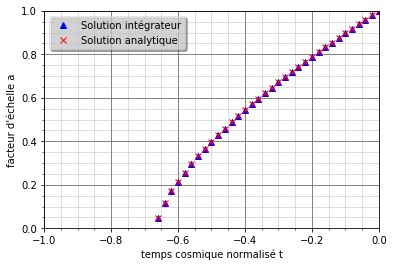
\includegraphics[width=8.0cm,height=6cm]{EDSf.png}
\caption{Univers Einstein-De Sitter}
\label{fig:UEDS}
\end{subfigure}
\begin{subfigure}{0.5\textwidth}
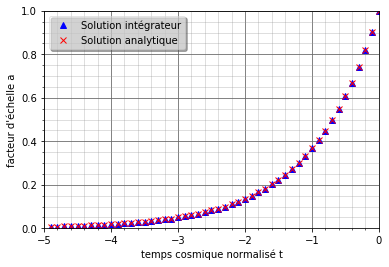
\includegraphics[width=8.0cm,height=6cm]{DSf.png}
\caption{Univers De Sitter}
\label{fig:UDS}
\end{subfigure}

\caption{Comparaison des solutions analytiques et intégrateur}
\label{fig:UISC}
\end{figure}

%\begin{comment}
\makeatletter
\renewcommand\chapter{\thispagestyle{plain}%
\global\@topnum\z@
\@afterindentfalse
\secdef\@chapter\@schapter}
\makeatother 
%\end{comment}

\section{Modèle simplifié inspiré du modèle $\Lambda$CDM}
$\Lambda$ est la constante cosmologique et CDM est l'acronyme de Cold Dark Matter. \begin{comment}C'est une théorie à paramètres. La fameuse matière noire n'est toujours pas identifiée. La valeur de la constante cosmologique est le résultat d'un ajustement. Néanmoins cette théorie permet d'expliquer avec une grande validité diverses constatations astrophysiques. Nous n'avons pas besoin d'en comprendre tous les détails pour poursuivre l'objectif de ce stage.\end{comment}

\subsection{Valeurs des paramètres par la mission Planck 2018}
Le tableau \ref{tab:PI} liste les valeurs utilisées dans notre modèle. Elles sont calculées ou prises dans le tableau 2 colonne "TT,TE,EE+lowE+lensing" du papier "Planck 2018 results. VI. Cosmological parameters"\textsuperscript{\cite{Planck2018}}.
\begin{table}
\begin{center}
\begin{tabular}{ m{5cm} m{5cm} } 
 \hline
 Paramètre & Valeur numérique\\ 
 \hline
$\Omega_\Lambda$ & 6.847e-1\\ 
$\Omega_m$ & 3.153e-1\\ 
$\Omega_{dm}$ & 2.660e-1\\ 
$\Omega_b$ & 4.93e-2\\ 
$\Omega_r$ & 9.28e-5\\
$\Omega_K$ & 0.000\\
$\Omega_\Lambda$ & 6.847e-1\\ 
$z_{eq}$ & 3.402e3\\
$T_0 [K]$ & 2.7255e0\\ 
$H_0 [km s^{-1} Mpc^{-1}]$ & 6.736e1\\ 
 \hline

\end{tabular}
\end{center}
\caption{Paramètres modèle $\Lambda$CDM simplifié}
\label{tab:PI}
\end{table}

\subsection{La constante cosmologique et l'énergie noire}
L'équation d'einstein avec constante cosmologique s'écrit:
\begin{equation} \label{eq:EFEL}
\boxed{R_{\mu \nu} \ - \ \frac{1}{2} \, g_{\mu \nu} \, R  \ + \ \Lambda \ g_{\mu \nu} \ =  \kappa T_{\mu \nu}}
\end{equation}
On peut cependant interpréter la constante cosmologique comme un fluide parfait de densité d'énergie positive constante qu'on appelle énergie noire et de pression négative avec pour équation d'état :
\begin{equation} \label{eq:EEL}
\boxed{P_\Lambda=-1 \times \rho_\Lambda}
\end{equation}
La méthode est de poser un nouveau tenseur énergie-impulsion qui inclut en son sein la constante cosmologique grâce à un changement de variable. On obtient finalement que la densité volumique d'énergie noire vaut :
\begin{equation} \label{eq:DEL}
\boxed{\rho_{\Lambda}  =  \frac{c^4 \Lambda}{8\pi G}}
\end{equation}

\subsection{La matière noire et baryonique froide}
La matière noire est supposée interagir uniquement par gravité. On suppute aussi qu'elle est froide de sorte que seule son énergie de masse compte pour le calcul de la densité d'énergie. 
Dans ce stage, la période d'intérêt fait que la température cinétique de la matière baryonique est constamment inférieure à 10 000K. Cette température est considérée comme froide en comparaison à l'énergie de masse. Pareillement à la température de la matière noire, la température baryonique n'intervient donc pas dans le calcul de la densité d'énergie, seule son énergie de masse compte. Cela revient à considérer que la matière est immobile et exerce une pression nulle.
En conséquence son équation d'état est :
\begin{equation} \label{eq:EEM}
\boxed{P_m=0 \times \rho_m c^2}
\end{equation}
avec $\rho_m$ la densité de masse de la matière noire et baryonique.
D'après \ref{eq:F3S}, on obtient que :

\begin{equation} \label{eq:DEM}
\boxed{\rho_{\rm m}(t) = \rho_{\rm m}(t_0) \left(\frac{a(t_0)}{a(t)}\right)^3}
\end{equation}

Cette dernière équation peut aussi se retrouver par un raisonnement sur la densité particulaire qui varie tel que 
\begin{equation} \label{eq:NP}
\boxed{n(t) = n(t_0) \left(\frac{a(t_0)}{a(t)}\right)^3}
\end{equation}

\subsection{Le champ de rayonnement électromagnétique et les neutrinos}
La découverte du fond diffus cosmologique a eu impact retentissant en cosmologie. Grâce à lui nous pouvons savoir notre vitesse par rapport à ce champ de rayonnement, définissant en quelque sorte un référentiel privilégié, fait rare en relativité générale. Ce "référentiel" n'est autre que celui de l'observateur cosmique ajoutant du crédit au principe cosmologique et à la métrique FLRW. 
\subsubsection{La température de radiation}
Le fond diffus est un rayonnement primordial qui s'est refroidi avec l'expansion et dont la distribution en fréquence se modélise comme un corps noir presque parfait de température T dont la distribution est donnée par la loi de planck. En plaçant des photons dans une cavité du vide de longueur L, on montre fortunément que le refroidissement adiabatique dû à l'expansion d'un corps noir est un corps noir de température amoindrie, de sorte que $T_r$ évolue en $T_{r0} (1+z)$:
\begin{equation} \label{eq:TRRA}
\boxed{T_r(t) = T_r(t_0) \frac{a(t_0)}{a(t)}}
\end{equation}

%\subsubsection{\uppercase{é}quation d'état}
Par le même raisonnement on montre que la densité d'énergie radiative évolue en $\rho_{r0} (1+z)^4$ :
\begin{equation} \label{eq:DER}
\boxed{\rho_r(t) = \rho_r(t_0)  \left({\frac{a(t_0)}{a(t)}}\right)^4}
\end{equation}

Avec la distribution de planck on trouve le tenseur énergie impulsion du champ radiatif et le résultat bien connnu que la pression radiative vaut le tiers de l'énergie radiative (pour un corps noir) :
\begin{equation} \label{eq:EER}
\boxed{P_r = \frac{1}{3} \times \rho_r}
\end{equation}
Grâce à l'équation d'état on peut utiliser \ref{eq:F3S} pour retrouver \ref{eq:DER} 

\subsubsection{Neutrinos}
Les neutrinos ont des masses nulles ou quasi-nulles et une vitesse égale ou proche de celle de la lumière. Ils peuvent être traités comme des photons, mais l'histoire de l'univers dans sa genèse fait que la densité d'énergie des neutrinos est moindre :

\begin{equation} \label{eq:EDN}
\boxed{\rho_n \approx 0.68 \times \rho_r}
\end{equation}
La prise en compte de la densité énergétique des neutrinos en sus des photons permet de trouver une bonne estimation de $\Omega_{ro}$.
\subsection{Intégrateur et solution simplifiée de l'expansion}
Au vu de ce qui a été dit depuis le début, l'équation de Friedmann 1 (\ref{eq:F1}) s'écrit pour nos conditions :

\begin{equation} \label{eq:ELCDM}
\boxed{a' = \sqrt{\Omega_{\Lambda}*a^2+\Omega_{m0}/a+\Omega_{ro}/a^2}}
\end{equation}
avec $a'$ la dérivée par rapport au temps cosmique normalisé. Le temps cosmique normalisé est le temps sans dimension : $t' = H_0 \times t$.  Le temps nul correspond à actuellement et le facteur d'échelle y est pris à 1. L'intégrateur remonte dans le temps. L'Univers survit une portion d'environ 0.95 du temps de Hubble. La figure \ref{fig:ULCDM} donne les résultats de notre intégrateur.

\begin{figure}[]
\centering
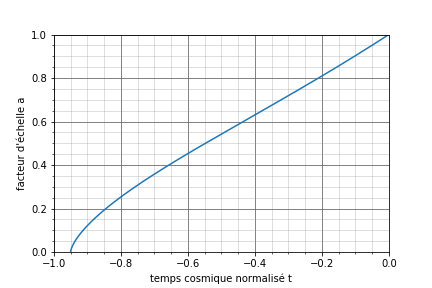
\includegraphics[width=12.0cm,height=9cm]{LCDMf.png}
\caption{Univers $\Lambda$CDM simplifié}
\label{fig:ULCDM}
\end{figure}
 

%\section{L'époque de recombinaison}
\section{\uppercase{é}changes d'énergie entre photons et électrons}
\subsection{La température baryonique}
On suppose que la matière interagit suffisament par collision pour justifier une hypothèse simplificatrice, celle d'une température baryonique $T_b$. Pleinement justifiée aux grands $z$, cette hypothèse n'est plus valable aux petits $z < 10$ où la densité et la température devient faible.
\subsubsection{Refroidissement adiabatique dû à l'expansion}
L'hypothèse de De Broglie est employée afin d'appliquer le même raisonnement que celui de la conservation des noeuds d'une longeur d'onde dans une cavité. Il vient que $T_b$ évolue en $T_{b0} (1+z)^2$:

\begin{equation} \label{eq:RTB}
\boxed{T_b(t) = T_b(t_0) \left(\frac{a(t_0)}{a(t)}\right)^2}
\end{equation}

\subsection{Processus Compton}
C'est le processus de diffusion d'un photon sur un électron libre, il a une importance capitale en cosmologie à cause de sa grande section efficace. La diffusion d’un photon sur un proton a quant à elle une section efficace environ mille fois plus faible et peut donc être négligée. On rappelle les résultats principaux. Dans le référentiel de l'électron au repos, le photon de longeur d'onde $\lambda$ arrivant sur l'électron définit une direction privilégiée. Dans cette configuration, l'électron ne peut que gagner de l'énergie. On note $\theta$ l'angle de déviation du photon par rapport à sa propre direction.
La variation de longeur d'onde vaut :
\begin{equation} \label{eq:VLO}
\boxed{\Delta\lambda=\frac{h}{m_e c}(1 - \cos \theta)}
\end{equation}

 Le premier ordre non trivial de l'électrodynamique quantique nous dit que la section efficace différentielle non polarisée vaut :
\begin{equation} \label{eq:QED}
\boxed{\frac{d\sigma}{d\Omega} = \frac{1}{2} r_e^2 \left(\frac{\lambda}{\lambda'}\right)^{2} \left[\frac{\lambda}{\lambda'} + \frac{\lambda'}{\lambda} - \sin^2(\theta)\right]}
\end{equation}

La diffusion Thompson est la limite basse énergie de la diffusion Compton. Dans cette approximation, le photon accélère une particule chargée qui rayonne. Ce rayonnement est alors interprété comme étant la diffusion du photon sur la particule chargée. 

\subsubsection{Processus Compton Inverse}
Si l'électron n'est pas au repos, on peut toujours faire un changement de référentiel pour avoir l'électron au repos et appliquer la théorie du processus Compton, puis faire un changement de référentiel inverse pour revenir au référentiel initial où l'électron se meut. L'électron ou le photon peut alors avoir gagné ou perdu de l'énergie.
%\subsubsection{Diffusion Thompson}


\subsection{Chauffage des électrons par les photons}

Pour calculer les échanges d'énergies à l'ordre zéro entre les températures baryoniques et de rayonnement, une approche simple mais controversée est utilisée. Un électron qui se meut à une vitesse non nulle par rapport à un champ de rayonnement de corps noir isotrope va percevoir une température de rayonnement plus forte pour les rayons venant à contresens et plus faible pour les rayons dans le même sens -- une manifestation de l'effet Doppler. Cette anisotropie a pour conséquence finale que l'électron est freiné et donc refroidi. On peut calculer ce refroidissement qui a le mérite de faire apparaître une expression homogène et les grandeurs appropriées. À partir de là, on "transforme ce refroidissement en réchauffement" afin d'obtenir un terme simple d'échange d'énergie entre photons et électrons : 
\begin{equation} \label{eq:ITBTR}
\boxed{\frac{dT_b}{dt} = \frac{8\sigma_Ta_rT_r^4(T_r-T_m)}{3m_ec}\frac{x_e}{1+x_e}}
\end{equation}

 où $\sigma_T$ est la section efficace de Thompson, $m_e$ la masse de l'électron, $a_r$ la constante de rayonnement et $x_e$ la fraction d'ionisation.

Du fait de cette interaction, la distribution en fréquence des photons n'est plus exactement celle d'un corps noir.   
 
\subsection{Fraction d'ionisation $x_e$}
Par définition :
\begin{equation} \label{eq:XE}
\boxed{x_e= \frac{n_e}{n_p+n_H}}
\end{equation}
On peut utiliser dans un premier temps la loi de Saha-Langmuir valable pour une ionisation faible :
\begin{equation} \label{eq:XESL}
\boxed{\frac{n_{i+1} n_e }{n_i} = \frac{2 Z_{i+1}}{Z_i} \left( \frac{2\pi m_ek_bT}{h^2}\right)^{\frac{3}{2}} \exp(\frac{-\chi_i}{k_bT})}
\end{equation}
Son utilisation ici est abusive car la fraction d'ionisation est proche de l'unité à 10000K pour l'hydrogène. Pour les résultats préliminaires il a été choisi de prendre une fraction d'ionisation constante égale à 4e-4\textsuperscript{\cite{Flower}}.

Où $\chi_i$ est le potentiel d'ionisation pour ioniser de nouveau un atome déjà ionisé $i$ fois, $Z_i$ est sa fonction de partition. Cette loi permet d'obtenir la fraction d'ionisation d'un gaz d'hydrogène à la température $T$ :
\begin{equation} \label{eq:XE}
\boxed{\frac{x^2}{1-x} = \frac{1}{n_p+n_H} \left( \frac{2\pi m_ek_bT}{h^2}\right)^{\frac{3}{2}} \exp(\frac{-13.6}{k_bT})}
\end{equation}

\subsection{Paramètre $z_{eq}$}
Par définition, il correspond au décalage vers le rouge cosmologique où la densité énergétique de rayonnement est égale à celle de la matière. Par conséquent, on obtient une autre estimation du paramètre $\Omega_{ro} = \frac{\Omega_{m}}{1+z_{eq}}$. $z_{eq} = 3402$ voir \ref{tab:PI}. La température baryonique est environ égale à la température de rayonnement car le terme compensateur Compton est très important : $T_b \approx T_r$ de sorte que l'on utilise cette condition intiale dans notre programme.

\subsection{Intégrateur et évolution des températrures}
On néglige pour l'instant l'interaction des photons avec les molécules et atomes. Au vu de ce qui a été dit, la température baryonique évolue comme :

\begin{equation} \label{eq:EERT}
\boxed{\frac{dT_b}{dt} = -2H(t)T_b+\frac{8\sigma_Ta_rT_r^4(T_r-T_m)}{3m_ec}\frac{x_e}{1+x_e}}
\end{equation}

et la température radiative comme :

\begin{equation} \label{eq:EERR}
\boxed{\frac{dT_r}{dt} = -H(t)T_r}
\end{equation}

La figure \ref{fig:T} résume les résultats de notre intégrateur pour différentes fractions d’ionisation supposées constantes en fonction de z.

\begin{figure}[]
\centering
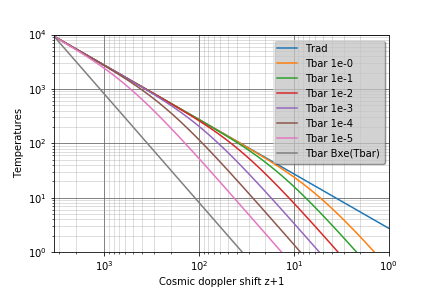
\includegraphics[width=12.0cm,height=9cm]{Temperatures.png}
\caption{\uppercase{é}volution des températures baryonique et de radiation pour différentes fraction d'ionisation}
\label{fig:T}
\end{figure}

\section{Refroidissement moléculaire}
\subsection{Généralités $\&$ réseau}
Les atomes et molécules considérés pour un modèle possèdent des états d'énergie interne outre leur énergie cinétique qui sont décrits par un certain jeu de nombres quantiques. Le but est de trouver la densité particulaire de chaque espèce dans chaque configuration quantique donnée. Cette dernière densité est aussi égale à la densité totale de l'espèce, fois sa proportion dans l'état quantique. Les densités sont décrites par des équations différentielles qui forment un réseau.\bigskip
\large

Listons les termes sources et dissipatifs susceptibles de faire varier les densités $\frac{dn_i}{dt}$ :\\

\begin{enumerate}
	\item Les désexcitations radiatives spontanées : $\sum\limits_{j>i} n_jA_{ji}-n_i\sum\limits_{j<i} A_{ij}$
	\item Les absorptions et les émissions stimulées : $\sum\limits_{j<i} n_jB_{ji}J_{ij}+\sum\limits_{j>i} n_jB_{ji}J_{ji}-n_i\sum\limits_{j<i}B_{ij}J_{ij}$
	\item Les excitations et désexcitations collisionnelles avec chaque collisionneur p : \\ $\sum\limits_p\left(\sum\limits_{j<i}n_p n_j C_{ji}-n_pn_i\sum\limits_j C_{ij}+n_p\sum\limits_{j>i}n_j C_{ji}\right)$
	\item Une dilution dû à l'expansion du volume : $-3Hn_i$\\
	\item Les termes de réactions chimiques formant ou détruisant l'espèce dans un état quantique donné.
\end{enumerate}
\medskip
\normalsize
La température radiative intervient dans l'expression des moyennes de l'intensité $J_{ij}$, tandis que la température baryonique intervient implicitement dans les taux de collisions $C_{ij}$. Les moyennes de l'intensité et le refroidissement dépendent de l'épaisseur optique de sorte qu'un code qui modélise le transfert de rayonnement est nécessaire. 
%\subsection{\uppercase{é}léments de transfert de rayonnement}
\subsection{Réchauffement/Refroidissement}
Nous ne pouvons définir une température thermodynamique de notre système global prenant en compte l'énergie potentielle des états internes et gravitationnels, l'énergie cinétique et l'énergie radiative. Par contre dans notre bulle d'effondrement, nous pouvons définir une température cinétique locale, celle de la distribution des vitesses de Maxwell relié à l'énergie cinétique volumique locale. On suppose que toutes les espèces possèdent la même température cinétique, l'hypothèse se justifie à l'aide de l'argument de la thermalisation de la matière, induite par collisions avec les électrons. 
\bigskip
\large

Listons les termes sources et dissipatifs susceptibles de faire varier l'énergie cinétique volumique locale $\frac{dE_{CV} }{dt}$ :\\

\begin{enumerate}
	\item La diffusion Compton, de manière générale, la diffusion des photons avec la matière baryonique (voir sections précédantes).
	\item Réchauffement par désexcitations collisionnelles avec chaque collisionneur p :\\ $\sum\limits_p\sum\limits_{j>i}\sum\limits_i n_p n_j C_{ji}E_{ji}$
	\item Refroidissement par excitations collisionnelles avec chaque collisionneur p :\\ $-\sum\limits_p\sum\limits_{j>i}\sum\limits_i n_p n_j C_{ij}E_{ij}$
	\item Perte d'énergie cinétique dû à l'expansion de la longueur d'onde (hypothèse de De Broglie): $-2H E_{CV}$
	\item Pertes volumiques dû à l'expansion du volume : $-3H E_{CV}$
	\item Les termes de réactions chimiques exo/endothermique provenant des créations/destructions de molécules.
	\item L'excès d'énergie éventuel lors des absorptions, qui se transforme en énergie cinétique ? rien trouvé sur le sujet. A supprimer probablement.
\end{enumerate}
\medskip
\normalsize
Les désexcitations radiatives interviennent indirectement en modifiant les populations et l'intensité radiative.
\subsection{Relation entre énergie cinétique et température cinétique}
Un calcul classique de théorie cinétique des gaz permet de relier l'énergie cinétique volumique $E_{CV}$ à la température cinétique $T_C$ des m espèces:
\begin{equation} \label{eq:ECTC}
 \boxed{E_{CV} = \sum\limits_m  \frac{3 n_i k_b T_C}{2}}
\end{equation}
Ainsi, grâce aux termes des listes précédantes, le nécessaire est là pour calculer la variation de la température cinétique des $m$ atomes/molécules :
\begin{equation} \label{eq:VTC}
 \boxed{\frac{dT_C }{dt} = \frac{d}{dt}\left(\frac{E_{CV}}{\sum\limits_m  \frac{3 n_i k_b}{2}}\right)}
\end{equation}


\subsection{Le programme RADEX}
RADEX\textsuperscript{\cite{RADEX}} est un programme livré avec le code source qui résout l'équilibre statique du réseau, i.e. avec les dérivées temporelles des densités particulaires nulles. Il modélise la partie transfert de rayonnement avec une probabilité d'échappement du photon. Le logiciel est capable de fonctionner sans équilibre thermodynamique local et peut prendre ainsi en compte une température radiative différente de la température baryonique. Il a déja fait ses preuves dans la communauté astrophysique et est utilisé dans ce stage.
\subsection{La molécule $H_2$}
La molécule est modélisée à l'ordre zéro comme un rotateur rigide -- deux protons fixés par une tige rigide -- et comme un oscillateur harmonique -- la tige est le ressort. Deux nombres quantiques décrivent les états d'énergie rotovibrationnel du système.  
\subsubsection{Forme ortho et para}
La molécule de dihydrogène possède deux isomères de spin nucléaire. Une configuration où les moments cinétiques intrinsèques des protons sont parallèles, la forme ortho, et une autre où ils sont anti-parralèlles, la forme para. En réalité cette description est trop simpliste, il faut avoir une approche de mécanique quantique avec le spin nucléaire total. Il y a deux cas possibles : le spin nucléaire total I vaut 1 dégénéré 3 fois avec une projection de la base de spins dans une direction quelquonque valant {-1,0,1} -- la forme ortho -- ou le spin nucléaire total I est nul et dégénéré une seule fois -- la forme para. Les transitions spontanées entre les deux formes sont fortement interdites -- les temps caractéristiques des ces transitions sont plus élevés que l'âge de l'univers. En revanche les dés/excitations collisionnelles réactives permettent de passer entre les deux formes. 
\subsubsection{Rapport ortho para}
Il est possible de calculer le rapport théorique ortho para pour du dihydrogène à l'équilibre thermodynamique à la température $T$ grâce à la loi de Boltzmann :
\begin{equation} \label{eq:EROP}
\boxed{r(o/p) = \frac{Z_o}{Z_p}}
\end{equation}
avec $Z$ la fonction de partition définie par :
\begin{equation} \label{eq:EZ}
 \boxed{Z = \sum\limits_i g(E_i) \ \exp\left(\frac{-E_i}{k_bT}\right)}
\end{equation}
 
$Z_o$ désignant alors la ponction de partition avec seulement les états d'énergie dans la forme ortho et $Z_p$ défini similairement avec la forme para.


\subsection{Intégrateur et rapport ortho para}

La figure \ref{fig:ROP} montre le rapport ortho-para calculé à différents $z$ grâce aux données déduites du modèle par l'intégrateur et au programme RADEX. RADEX prend en arguments d'entrée les températures calculées par l'intégrateur ainsi que les densités de collisionneurs. Il s'agit ici des protons et des atomes d'hydrogène. RADEX a aussi besoin d'un fichier d'information sur la molécule $H_2$ et les collisionneurs lui indiquant les niveaux d'énergies et les taux de collisions calculés à différentes températures. La densité des atomes d'hydrogène a été prise en considérant que l'ensemble de la matière baryonique est sous forme d'atomes d'hydrogène, ainsi :
\begin{equation} \label{eq:NHT0}
 \boxed{n_H(t_0) = \frac{\Omega_{b} \rho_c}{m_H c^2} }  
\end{equation}
et
\begin{equation} \label{eq:NH}
\boxed{n_H(t) = n_H(t_0) \left(\frac{a(t_0)}{a(t)}\right)^3 } 
\end{equation}


\begin{figure}[]
\centering
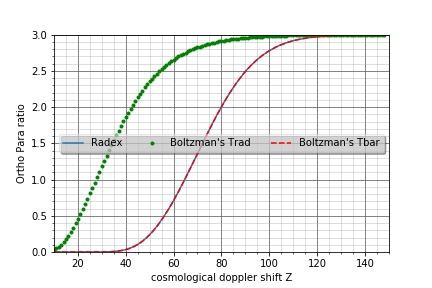
\includegraphics[width=14.0cm,height=9cm]{rop.png}
\caption{Rapport ortho para}
\label{fig:ROP}
\end{figure}

La série de points verts Boltzmann $T_r$ correspond au rapport théorique qu'on obtiendrait avec Boltzmann en prenant la température radiative $T=T_r(z)$.
La série de tirets oranges Boltzmann $T_b$ correspond au rapport théorique qu'on obtiendrait avec Boltzmann en prenant la température baryonique $T=T_b(z)$.
Enfin les points rouges correspondent à la courbe obtenue par Flower et Pineau des forêts dans leur modèle. 
Leur rapport ne descend pas vers zéro. L’explication découle du fait qu’ils ne résolvent pas les équations de l’équilibre statique, i.e. ils ne supposent pas un état stationnaire à chaque z et résolvent l’équilibre statistique dépendant du temps. Aux faibles $z$, quand la densité devient faible, elle peut descendre en dessous de la densité critique de transfert de rayonnement -- les désexcitations collisionnelles devenant plus rares que les désexcitations spontanées. Ainsi les populations de l'équilibre statique que l'on calcule avec RADEX n'ont jamais le temps de s'établir, c'est pourquoi le rappport ortho para semble geler vers une valeur non nulle (de l’ordre de 0.3) avec leur modèle. Les différences aux $z \approx 50 - 100$ sont par contre la conséquence d'un modèle physique différent : pas de $\Lambda CDM$, paramètres non égaux, etc...

\addcontentsline{toc}{chapter}{Conclusion} 
\section*{Conclusion}
Notre équipe s'est formée et a compris dans l'ensemble le modèle $\Lambda CDM$. Bien connaître son sujet était un objectif préalable avant toute modélisation. Un intégrateur avec un modèle $\Lambda CDM$ simplifié a ensuite été développé. Il fourni le facteur d'échelle en fonction du temps ainsi que les températures radiatives et baryoniques. Ces dernières, avec les densités particulaires sont les variables d'importance pour étudier la chimie. Le programme RADEX a ensuite été utilisé pour résoudre les populations de l'équilibre statique de la molécule $H_2$. Dans la suite du stage il est prévu :

\begin{itemize}
	\item [$\bullet$] Mettre à jour les résultats préliminaires avec la fraction d'ionisation résultant de la loi de Saha
	\item [$\bullet$] Augmenter la taille du réseau avec l'ajout de la molécule HD par exemple
	\item [$\bullet$] Mettre à jour les fichiers de collisions
	\item [$\bullet$] Préciser les termes de création et de destruction de molécules, i.e. avoir un modèle de chimie réaliste
	\item [$\bullet$] Avoir une formule moins controversée et plus réaliste pour le terme d'interaction Thompson photons-électrons. 
	\item [$\bullet$] Faire un code similaire à RADEX dans la modélisation du transfert de rayonnement et de son caractère non LTE mais donnant les populations hors équilibre statique
	\item [$\bullet$] Prendre en compte les interactions avec les molécules dans l'équation d'évolution de la température baryonique 
\end{itemize}

Ceci nous permettra de calculer les densités particulaires et non seulement les rapport ou les proportions de populations afin de pouvoir calculer précisément le refroidissement.

S'il reste du temps, il est enfin prévu de réaliser l'objectif initial, c'est à dire la modélisation de l'effondrement menant aux étoiles POP III. C'est une modélisation pleine de défis. Afin de rester réaliste dans ses ambitions, un modèle 2D non turbulent d'une bulle de gaz dépendant d'un rayon et du temps sera probablement implémenté. L'amélioration continuelle de la puissance de calcul des processeurs joue en notre faveur. 

\appendix

\chapter{Intégrateur et Programmes}
L'ensemble des codes (C, python) et ressources (pdf, code latex, images...) sont disponibles sur la page \url{https://github.com/ANDREMIV/stageM2}

L'intégrateur est une implémentation de la méthode Runge-Kutta d'ordre 6 en C. Les résultats sont ensuite mis en forme par des scripts python via la bibliothèque matplotlib. 

%\section{Formules utiles de Transfert de Rayonnement}
%\section{Le programme Radex}
\begin{comment}
\makeatletter
\renewcommand\chapter{\if@openright\cleardoublepage\else\clearpage\fi
\thispagestyle{plain}%
\global\@topnum\z@
\@afterindentfalse
\secdef\@chapter\@schapter}
\end{comment}

\begin{thebibliography}{}

\bibitem{Coppola} 
The chemistry of the early Universe, Carla Marla Coppola and Daniele Galli
\\doi:10.1088/2514-3433/aae1b5ch1

\bibitem{Flower} 
The ortho:para $H_2$ ratio in the primordial gas, D. R. Flower and G. Pineau des Forêts
\\Mon. Not. R. Astron. Soc. 316, 901-905 (2000)

\bibitem{Galli} 
The Dawn of Chemistry, Daniele Galli and Francesco Palla
\\doi:10.1146/annurev-astro-082812-141029

\bibitem{Planck2018} 
Planck 2018 results. VI. Cosmological parameters
\\\url{https://arxiv.org/pdf/1807.06209.pdf}

\bibitem{Weinberg} 
Cosmology, Steven Weinberg

\bibitem{Signes}
Conventions de Signes RG
\\\url{https://en.wikipedia.org/wiki/Einstein_field_equations#Sign_convention}

\bibitem{cours_RG1} 
Relativité Générale, cours de M2, Éric Gourgoulhon
\\\url{https://luth.obspm.fr/~luthier/gourgoulhon/fr/master/relatM2.pdf}

\bibitem{cours_RG2} 
INTRODUCTION A LA RELATIVITE GENERALE, Luc Blanchet
\\\url{http://www2.iap.fr/users/blanchet/images/coursRG.pdf}

\bibitem{RADEX} 
RADEX
\\\url{https://arxiv.org/pdf/0704.0155.pdf}



\end{thebibliography}


\end{document}